\chapter{Background}\label{background}

This chapter provides an in-depth overview of the Transformer architecture, focusing on its core components, different variants, positional encoding schemes, and the processes of training and inference.

\section*{Notation}\label{sec:notation}

\begin{center}
    \begin{tabular}{cl}
        $\mathcal{V}$ \qquad & Vocabulary of input tokens.                                                          \\
        $n$                  & Length of the input sequence.                                                        \\
        $b$                  & Batch size for batched input sequences.                                              \\
        $\mathbf{x}$         & Input sequence of tokens, $\mathbf{x} \in \mathcal{V}^{n}$                           \\
        $x_i$                & $i$-th token in the input sequence, $x_i \in \mathcal{V}$.                           \\
        $d$                  & Dimensionality of the token embedding space.                                         \\
        $\mathbf{e}_i$       & $d$-dimensional embedding vector of token $x_i$, $\mathbf{e}_i \in \mathbb{R}^d$.    \\
        $\mathbf{E}$         & Embedding matrix, $\mathbf{E} \in \mathbb{R}^{|\mathcal{V}| \times d}$.              \\
        $\mathbf{H}$         & Matrix of a sequence of embedding vectors, $\mathbf{H} \in \mathbb{R}^{n \times d}$. \\
        $\mathbf{h}_i$       & $i$-th vector in the sequence of embeddings, $\mathbf{h}_i \in \mathbb{R}^d$.        \\
        $\mathbf{O}$         & Output matrix from a Transformer layer, $\mathbf{O} \in \mathbb{R}^{n \times d}$.    \\
        $\mathbf{Q}$         & Queries matrix, $\mathbf{Q} \in \mathbb{R}^{n \times d}$.                            \\
        $\mathbf{K}$         & Keys matrix, $\mathbf{K} \in \mathbb{R}^{n \times d}$.                               \\
        $\mathbf{V}$         & Values matrix, $\mathbf{V} \in \mathbb{R}^{n \times d}$.                             \\
        $\theta$             & Model parameters (weights and biases).                                               \\
    \end{tabular}
\end{center}

\section{Transformer}\label{sec:transformer_arch}

The Transformer architecture, introduced by \textcite{vaswani_attention_2017}, performs sequence modeling by relying entirely on self-attention mechanism, instead of using convolution or recurrence.

Let $\mathcal{V}$ denote the vocabulary of input tokens. While the tokens can represent anything, in language modeling tasks they are usually learned subword units. In this work, however, a simple character tokenization scheme is used that is suitable for algorithmic tasks, so each token corresponds to a single character (letter, digit or symbol) in the sequence. An input sequence is represented as $\mathbf{x} = [x_1, x_2, \dots, x_n]$, where $x_i \in \mathcal{V}$ and $n$ is the sequence length. Each token $x_i$ is mapped to a $d$-dimensional embedding vector $\mathbf{e}_i \in \mathbb{R}^d$ using an embedding matrix $\mathbf{E} \in \mathbb{R}^{|\mathcal{V}| \times d}$. Thus, each row of $\mathbf{E}$ corresponds to the embedding of a token in the vocabulary.

The input matrix to a Transformer layer is a sequence of vector embeddings (also called the \emph{latent} or \emph{hidden representation} for intermediate layer inputs), denoted $\mathbf{H} \in \mathbb{R}^{n \times d}$, where $\mathbf{H} = [\mathbf{h}_1^\top, \mathbf{h}_2^\top, \dots, \mathbf{h}_n^\top]^\top$. The output of a Transformer layer is also a sequence of vectors with the same sequence length, denoted $\mathbf{O} \in \mathbb{R}^{n \times d}$.

In practice, the inputs to the Transformer are batched, so the input has an additional dimension for the batch size, denoted $b$, with $\mathbf{H} \in \mathbb{R}^{b \times n \times d}$. This results in the first (batch) dimension being added throughout the intermediate representation and the output, but has no bearing on the description of the Transformer model.

\subsection{Elements}\label{subsec:elements_transformers}

The Transformer is composed of several key components to model dependencies in sequential data: multi-head attention, feed-forward networks, layer normalization, and residual connections. Informally, the attention mechanism transfers information \emph{between} tokens, while the feed-forward networks process information \emph{within} tokens. These components are stacked in each layer of the Transformer as shown in Figure \ref{fig:transformer_layer} (a).

\paragraph{Attention Mechanism}

The attention mechanism \parencite{bahdanau_neural_2014} allows the model to weigh the relevance of different positions in the input sequence. For this purpose, it computes \emph{queries}, \emph{keys}, and \emph{values} from the input embeddings and uses them to calculate attention scores. The output is a weighted sum of the values, where the weights are determined by the attention scores. The names ``queries'', ``keys'', and ``values'' are derived from the context of information retrieval, where the queries are the elements being searched for, the keys are the elements being searched, and the values are the elements being retrieved. In the context of the Transformer, intuitively, the query represents what the current token is ``looking for'' in the sequence, the keys represent what the token at a given position ``offers'' to the current token, and the values are the actual information that the current token ``receives'' from the other tokens.

First, the queries, keys, and values are computed as:
\begin{align*}
    \mathbf{Q} & = \mathbf{H} \mathbf{W}^Q, \\
    \mathbf{K} & = \mathbf{H} \mathbf{W}^K, \\
    \mathbf{V} & = \mathbf{H} \mathbf{W}^V,
\end{align*}
where $\mathbf{W}^Q, \mathbf{W}^K, \mathbf{W}^V \in \mathbb{R}^{d \times d_k}$ are the weight matrices, and $d_k$ is the dimension of the queries, keys, and values. In practice, the convention is to set $d_k = d$, which is the case for the models in this work. Thus, $\mathbf{Q}, \mathbf{K}, \mathbf{V} \in \mathbb{R}^{n \times d}$.

Given queries $\mathbf{Q}$, keys $\mathbf{K}$, and values $\mathbf{V}$, the attention output is computed as:
\begin{equation*}
    \mathbf{O_{att}} = \text{Attention}(\mathbf{Q}, \mathbf{K}, \mathbf{V}) = \text{softmax}\left( \frac{\mathbf{Q} \mathbf{K}^\top}{\sqrt{d}} \right) \mathbf{V}.
\end{equation*}
where the softmax function is applied along the last dimension, and is defined as:
\begin{equation*}
    \text{softmax}(\mathbf{x})_i = \frac{e^{x_i}}{\sum_j e^{x_j}}.
\end{equation*}

Note that the output of the attention mechanism has the same shape as the input, $\mathbf{O_{att}} \in \mathbb{R}^{n \times d}$.

\paragraph{Multi-Head Attention}

Multi-head attention extends the attention mechanism with multiple independent \emph{heads} to allow the model to focus on information from different representation subspaces. So, instead of applying attention to the $d$-dimensional queries, keys, and values directly, they are projected into $h$ different $d_{head}$-dimensional subspaces, where $h$ is the number of heads. In this work, the head dimension $d_{head}$ is set to $d/h$, so that the total dimensionality remains $d$. The outputs the heads are concatenated and linearly transformed to the original dimensionality:
\begin{equation*}
    \text{MultiHeadAttention}(\mathbf{Q}, \mathbf{K}, \mathbf{V}) = \text{Concat}(\text{head}_1, \text{head}_2, \dots, \text{head}_h) \mathbf{W}^O,
\end{equation*}
where $\mathbf{W}^O \in \mathbb{R}^{d \times d}$ is the learned output weight matrix, and each head is computed as:
\begin{equation*}
    \text{head}_i = \text{Attention}(\mathbf{Q} \mathbf{W}_i^Q, \mathbf{K} \mathbf{W}_i^K, \mathbf{V} \mathbf{W}_i^V),
\end{equation*}
and $\mathbf{W}_i^Q, \mathbf{W}_i^K, \mathbf{W}_i^V \in \mathbb{R}^{d \times d_{head}}$ are the weight matrices for the $i$-th head.

\paragraph{Feed-Forward Networks}

Position-wise feed-forward networks (FFN), also called the Multi-layer Perceptron (MLP), are applied independently to each position in the sequence:
\begin{equation*}
    \text{FFN}(\mathbf{h}_i) = \sigma(\mathbf{h}_i \mathbf{W}_1 + \mathbf{b}_1) \mathbf{W}_2 + \mathbf{b}_2,
\end{equation*}
where $\mathbf{h}_i \in \mathbb{R}^d$ is the input vector, $\mathbf{W}_1 \in \mathbb{R}^{d \times d_{\text{ff}}}$, $\mathbf{W}_2 \in \mathbb{R}^{d_{\text{ff}} \times d}$, and $\sigma$ is an activation function such as Rectified Linear Unit (ReLU).

\paragraph{Layer Normalization}

Layer normalization \parencite{ba_layer_2016} is applied after each sub-layer over the last (feature) dimension. The $\text{LayerNorm}$ function for a vector $v \in \mathbb{R}^d$ is defined as:
\begin{equation*}
    \text{LayerNorm}(v) = \frac{v - \mu}{\sigma}\gamma + \beta,
\end{equation*}
where the scale $\gamma$ and bias vector $\beta$ are learned scaling and shifting parameters, and $\mu$ and $\sigma$ are the mean and standard deviation of $v$,computed as follows:
\begin{align*}
    \mu    & = \frac{1}{d} \sum_{i=1}^{d} v_i,                  \\
    \sigma & = \sqrt{\frac{1}{d} \sum_{i=1}^{d} (v_i - \mu)^2}.
\end{align*}

\paragraph{Residual Connections}

Residual connections \parencite{he_deep_2016} are usually applied to ease gradient flow and enable the training of deeper networks. In Transformer models, the residual connections are applied after each sub-layer (self-attention and MLP), followed by a layer normalization. Thus, the output of each sub-layer is:
\begin{equation*}
    \text{SubLayerOutput} = \text{LayerNorm}(\mathbf{x} + \text{SubLayer}(\mathbf{x})).
\end{equation*}

The residual connections-based view of the model also enables the concept of a \emph{residual stream}, which is important in mechanistic interpretability. In this alternative view of the model, the residual connections are the main backbone of information flow through the model, with the sub-layers processing the hidden representation tensor $\mathbf{H}$ and adding it back to the residual stream.

\paragraph{Block Structure}

The original Transformer introduced in \cite{vaswani_attention_2017} consists of stacked encoder and decoder blocks, each containing multi-head attention and feed-forward networks, along with residual connections and layer normalization. However, different modified architectures have been proposed, such as the encoder-only BERT model \parencite{devlin_bert_2019} and the decoder-only GPT model \parencite{radford_improving_2018}.

\begin{figure}[h!]
    \centering
    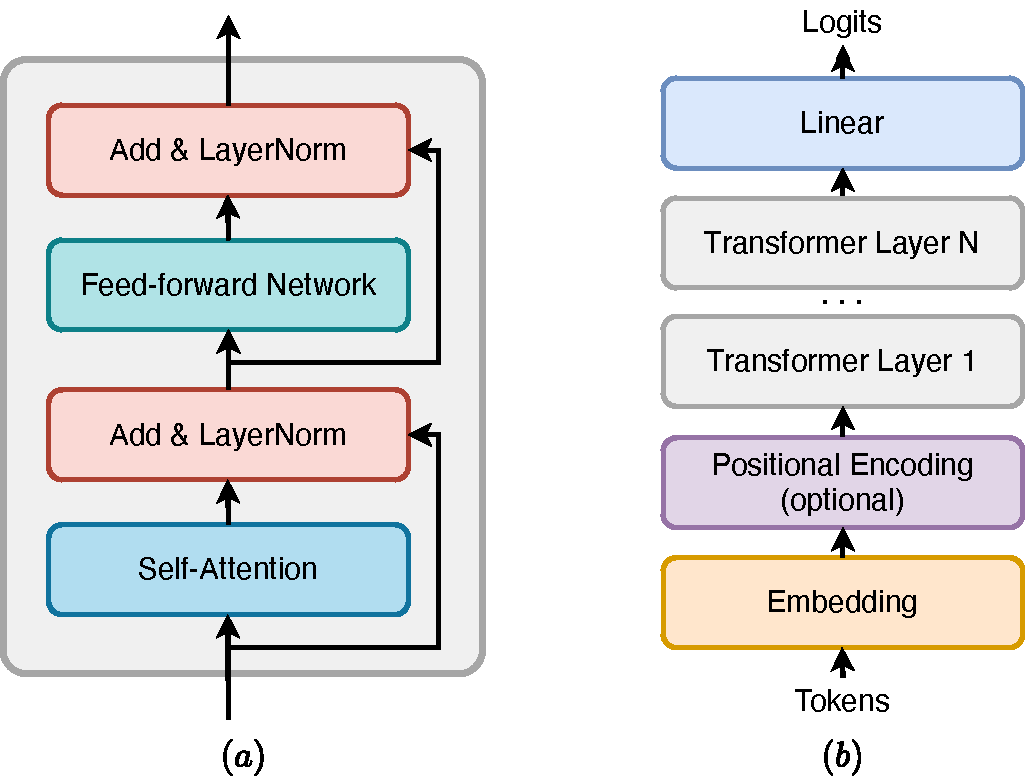
\includegraphics[width=0.8\textwidth]{fig/transformer_layer.pdf}
    \caption{(a) A single Transformer layer, consisting of multi-head self-attention, feed-forward network (MLP), and layer normalization. (b) A decoder-only transformer model. In the decoder, the self-attention mechanism has a causal mask to prevent attending to future tokens.}
    \label{fig:transformer_layer}
\end{figure}


\subsection{Encoder and Decoder Architectures}\label{subsec:types_transformers}

\TODO{overview}

\paragraph{Encoder-Decoder}

The original Transformer model introduced by Vaswani et al.~\cite{vaswani_attention_2017} employs an encoder-decoder architecture. In this architecture, the encoder processes an input sequence $\mathbf{x} = (x_1, x_2, \dots, x_n)$ into a sequence of continuous representations $\mathbf{z} = (z_1, z_2, \dots, z_n)$. The decoder then generates an output sequence $\mathbf{y} = (y_1, y_2, \dots, y_m)$ by predicting the next token $y_t$ based on the encoder's output and the previously generated tokens.

The encoder consists of a stack of $N$ identical layers, each containing two sub-layers: a multi-head self-attention mechanism and a position-wise fully connected feed-forward network. The decoder has a similar structure but includes a third sub-layer: the \emph{cross-attention}, also called \emph{encoder-decoder attention}, where the queries come from the previous decoder layer, and the keys and values come from the output of the encoder. Hence, the difference between the self-attention and cross-attention mechanisms is that self-attention is usually applied to the same sequence, while cross-attention is applied between two different sequences (e.g. one from the encoder, and one from the decoder). Moreover, the self-attention mechanism in the decoder has a causal mask to prevent attending to ``future tokens'', ensuring output is generated autoregressively.

\paragraph{Encoder-only}

Encoder-only models focus exclusively on encoding the input sequence into a contextual representation without a decoder component. BERT (Bidirectional Encoder Representations from Transformers)~\cite{devlin_bert_2019} is a prominent example of this architecture. BERT utilizes a stack of Transformer encoder layers to produce deep bidirectional representations by jointly conditioning on both left and right context. This makes encoder-only models particularly well-suited for tasks that require a comprehensive understanding of the input, such as text classification, named entity recognition, and question answering.

These models are typically pre-trained on large unlabeled text corpora using self-supervised objectives like masked language modeling (MLM) and next sentence prediction (NSP). The pre-trained models can then be fine-tuned on specific downstream tasks.

\paragraph{Decoder-only}

Decoder-only models generate sequences based on prior tokens and are designed primarily for autoregressive language modeling and text generation tasks. GPT (Generative Pre-trained Transformer)~\cite{radford_improving_2018} is a canonical example of a decoder-only architecture. In these models, the Transformer decoder predicts the next token in a sequence by attending to the previous tokens without an encoder component. Recent research on language modeling has mostly focused decoder-only models, since they can also be used on other language tasks through prompting, few-shot learning, and fine-tuning.

Decoder-only models are pre-trained on large text corpora to predict the next token, enabling them to generate coherent and contextually relevant text.

\bigskip

\paragraph{Encoder-Decoder vs. Decoder-Only} Both model types are capable of autoregressive sequence generation and can be used for a wide range of tasks. The decoder-only models are favored in recent works due to them being simpler and having less inductive bias. However, encoder-decoder models are still widely used in machine translation, robotics, and multi-modal learning tasks. The additional structure in encoder-decoder models, as compared to using a decoder-only model with would-be encoder input sequence prepended to the decoder's input can be summarized as:
\begin{itemize}
    \item The input to the encoder passes through more layers (encoder layers) before reaching the decoder.
    \item It is assumed that input and output sequences are sufficiently different to justify using separate parameters for them (encoder and decoder).
\end{itemize}

In summary, the choice of Transformer architecture depends on the specific requirements of the task, though decoder-only models have been more widely used in recent research and are the focus of this work.

\subsection{Recurrent and Looping Architectures}\label{subsec:recurrent_looping}

To enhance length generalization, some Transformers incorporate recurrence or looping mechanisms.

\paragraph{Universal Transformer}

The Universal Transformer \cite{dehghani_universal_2018} introduces recurrence into the Transformer architecture by repeatedly applying the same transformer layers multiple times:
\begin{equation*}
    \mathbf{H}^{(t+1)} = \text{TransformerLayer}(\mathbf{H}^{(t)}),
\end{equation*}
where $t$ denotes the iteration step. This enables the model to generalize better to sequences longer than those seen during training.

\paragraph{Looped Transformer}

\begin{figure}[h!]
    \centering
    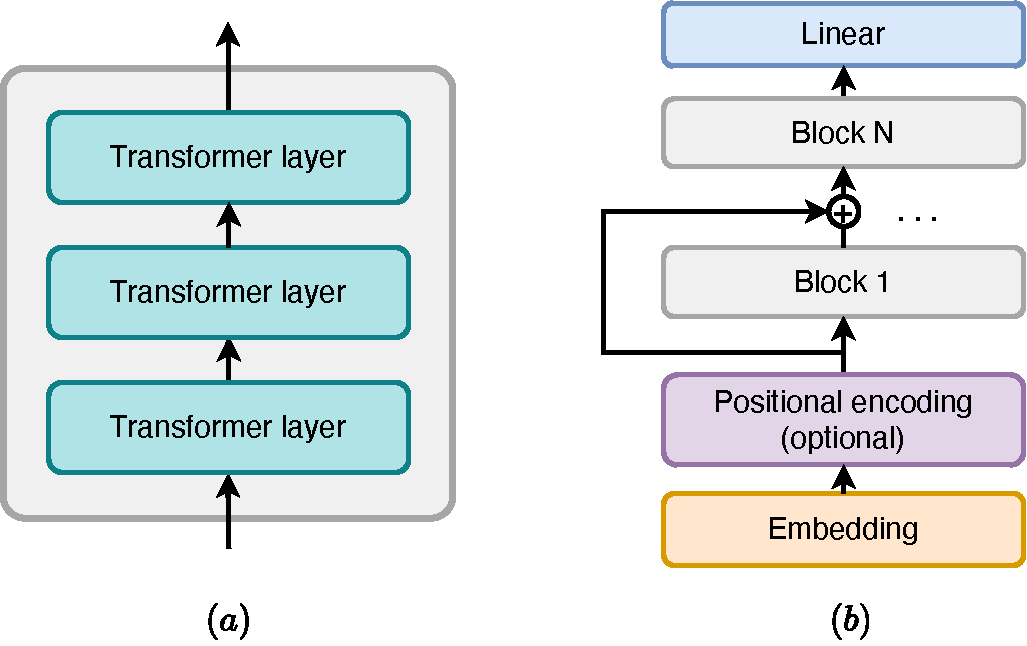
\includegraphics[width=0.8\textwidth]{fig/looped_transformer.pdf}
    \caption{(a) A block of multiple transformer layers used in the looped transformer. (b) Looped decoder-only transformer architecture. The input injection mechanism adds skip connections from the input sequence to the input of each block.}
    \label{fig:looped_transformer}
\end{figure}

Looped Transformers \parencite{yang_looped_2023} extend the Transformer by incorporating iterative application of a block of transformer layers.

\subsection{Positional Encoding Schemes}\label{subsec:positional_encoding}

Since the Transformer lacks inherent sequential order, positional encodings are added to input embeddings to provide position information. Though, several recent works have shown that the causal attention mechanism in a decoder-only transformer can also implicitly learn to encode positional information \parencite{zuo_breaking_2024,zhou_transformers_2024} in the absence of explicit positional encodings.

\paragraph{Sinusoidal Positional Encoding}\label{subsec:sinusoidal_pos_enc}

The original Transformer uses sinusoidal positional encodings \cite{vaswani_attention_2017}, defined as:
\begin{align*}
    \mathbf{p}_{i,2k}   & = \sin\left( \frac{i}{10000^{2k/d}} \right), \\
    \mathbf{p}_{i,2k+1} & = \cos\left( \frac{i}{10000^{2k/d}} \right),
\end{align*}
for position $i$ and dimension $k$. These encodings allow the model to generalize to longer sequences by extrapolating the sinusoidal patterns.

\paragraph{Relative Position Representations}\label{subsec:relative_pos_rep}

Relative position representations \cite{shaw_self-attention_2018} encode the relative distances between sequence elements directly into the attention mechanism. The attention scores are modified as:
\begin{equation*}
    e_{ij} = \frac{\mathbf{q}_i^\top \mathbf{k}_j + \mathbf{q}_i^\top \mathbf{a}_{i-j}^K + \mathbf{b}_{i-j}^Q{}^\top \mathbf{k}_j}{\sqrt{d_k}},
\end{equation*}
where $\mathbf{a}_{i-j}^K$ and $\mathbf{b}_{i-j}^Q$ are learned relative position embeddings.

\paragraph{Rotary Position Encoding (RoPE)}\label{subsec:rope}

RoPE \cite{su_roformer_2024} encodes positions using rotation matrices and incorporates relative position information into the self-attention mechanism. For each position $i$, the embedding is rotated by a position-dependent angle:
\begin{equation*}
    \mathbf{h}_i = \mathbf{e}_i \cdot \mathbf{R}(i),
\end{equation*}
where $\mathbf{R}(i)$ is a rotation matrix function of position $i$.

\paragraph{Randomized Positional Encodings}\label{subsec:random_pos_enc}

Randomized positional encodings \cite{ruoss_randomized_2023} aim to improve length generalization by simulating longer sequences during training. They randomly select a subset of positions to represent the sequence, enhancing the model's ability to handle sequences of unseen lengths.

\paragraph{Attention with Linear Biases (ALiBi)}\label{subsec:alibi}

ALiBi \cite{press_train_2021} introduces a linear bias to the attention scores based on the relative positions:
\begin{equation*}
    e_{ij} = \frac{\mathbf{q}_i^\top \mathbf{k}_j}{\sqrt{d_k}} + m \cdot |i - j|,
\end{equation*}
where $m$ is a head-specific constant slope parameter. This bias encourages the model to focus on recent tokens and enables better extrapolation to longer sequences.

\subsection{Training and Inference}\label{subsec:training_inference}

\TODO{diagram}


\begin{figure}[h!]
    \centering
    % 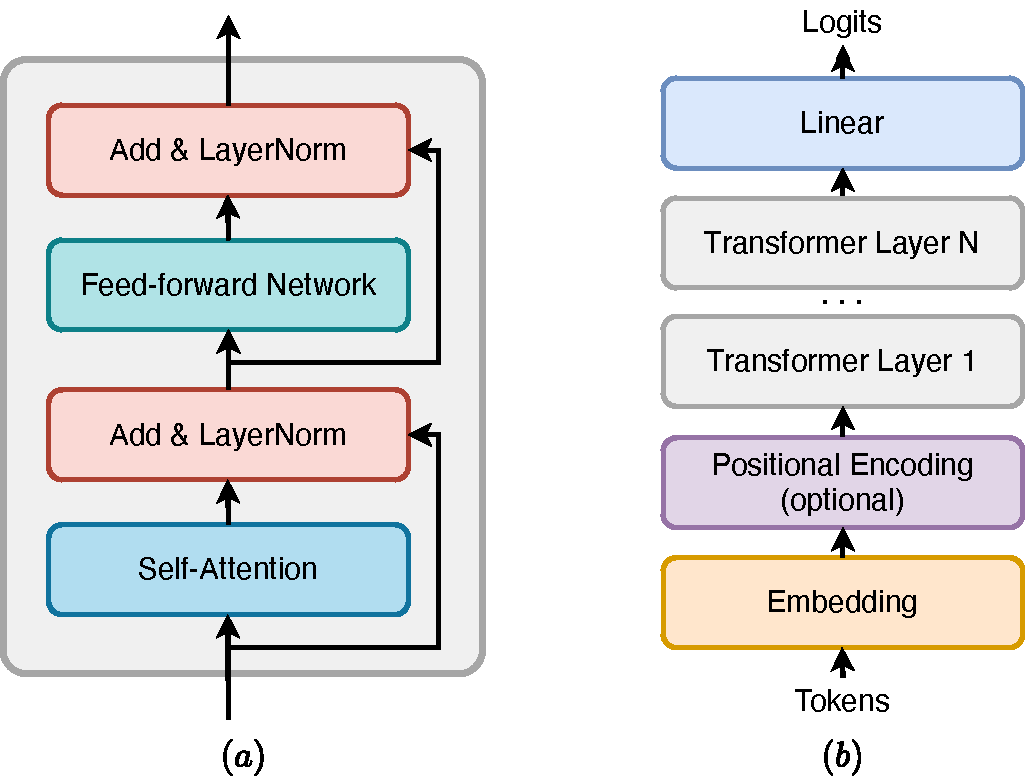
\includegraphics[width=0.8\textwidth]{fig/transformer_layer}

    % placeholder square before I have the actual diagram:
    \begin{tikzpicture}
        \node[draw, minimum width=0.7\linewidth, minimum height=6cm, color=red] (transformer_layer) {Transformer training and inference};
    \end{tikzpicture}

    \caption{Training and inference processes for Transformers TODO TODO TODO TODO.}
    \label{fig:transformer_training_inference}
\end{figure}

\paragraph{Training}

Training involves minimizing a loss function, typically the \emph{cross-entropy loss} for language tasks, using an optimization algorithm like Stochastic Gradient Descent (SGD) or AdamW \parencite{loshchilov_decoupled_2018}. The model learns the parameters $\theta$ by backpropagating the loss through the network layers. The cross-entropy loss is defined as:
\begin{equation*}
    \mathcal{L} = -\frac{1}{b} \sum_{i=1}^{b} \sum_{j=1}^{n} \log p(x_{i,j} | x_{i,<j}),
\end{equation*}
where $b$ is the batch size, $n$ is the sequence length, and $p(x_{i,j} | x_{i,<j})$ is the probability of token $x_{i,j}$ given the previous tokens $x_{i,<j}$.

\TODO{describe answer-only loss}

\paragraph{Inference}

During inference, the trained model generates outputs by computing the forward pass through the network. For autoregressive models, techniques like beam search may be used to generate sequences.



\section{Mechanistic Interpretability}\label{sec:mech_interp}

\TODO{expand}

Understanding how Transformers make decisions is crucial for interpretability and debugging. Key concepts include:

\paragraph{Residual Stream}

The residual stream in a Transformer accumulates information across layers through residual connections. Analyzing this stream helps in understanding how information is propagated and transformed.

\paragraph{Activation Patching}

Activation patching involves replacing activations in a model with activations from a different context to study causal effects \parencite{olsson_-context_2022}. This technique can identify which components contribute to specific model behaviors.

\paragraph{Logit Lens}

The logit lens method inspects the logits (pre-softmax outputs) at different layers to interpret intermediate representations. It provides insights into how predictions evolve across layers.

\textcite{olsson_-context_2022} investigated "induction heads," attention heads that enable in-context learning by recognizing patterns like repeated sequences.

\section{Realizability}\label{sec:realizability}

\TODO{maybe rename, fill, RASP/RASP-L and  Ahuja and Mansouri paper}

\section{Deep Double Descent}\label{sec:deep_double_descent}

The phenomenon of \emph{deep double descent} refers to the observation that increasing model capacity or training epochs can initially degrade performance before improving it \parencite{nakkiran_deep_2021}. This challenges the traditional bias–variance trade-off, where increasing complexity always leads to overfitting.

\textcite{belkin_reconciling_2019} explored this phenomenon, showing that modern machine learning models can benefit from overparameterization, achieving better generalization even when they perfectly fit the training data.

Understanding deep double descent is important for training Transformers effectively, as it informs decisions about model size and training duration to optimize performance on tasks like integer addition.

\TODO{explain why I care about this}